\documentclass[12pt, a4paper, twoside]{article}

\usepackage[utf8]{inputenc}
\usepackage[T1]{fontenc}
\usepackage[english]{babel}

%\usepackage{layout}
%\usepackage{geometry}
%\usepackage{setspace}
\usepackage{soul}
\usepackage{ulem}
%\usepackage{eurosym}

%\usepackage{bookman}
%\usepackage{charter}
%\usepackage{newcent}
%\usepackage{lmodern}
%\usepackage{mathpazo}
%\usepackage{mathptmx}

%\usepackage{url}
%\usepackage{verbatim}
%\usepackage{moreverb}
%\usepackage{listings}
%\usepackage{fancyhdr}
%\usepackage{wrapfig}
%\usepackage{color}
%\usepackage{colortbl}

\usepackage{amsmath}
\usepackage{amssymb}
\usepackage{mathrsfs}
%\usepackage{asmthm}

%\usepackage{makeidx}

\usepackage{graphicx}
\usepackage{caption}

\title{\huge{\textbf{Eye-Assisted Text Editing }\\ Future User Interfaces}}
\author{Gwenael \textsc{Gendre}, Lionel \textsc{Ieri}, Romain \textsc{Maillard} \\
	Teacher: Prof. Dr. Denis \textsc{Lalanne}}
\date{Summer 2018}
 
\begin{document}
 
\begin{titlepage}
\maketitle
\end{titlepage}
\tableofcontents
\newpage

\section{Introduction}
\textit{un peu bidon, ptet a changer? mais garder Logitech?}}
During the \textit{Future User Interfaces} course at the University of Fribourg, we had to develop and implement a multimodal interface, using eye tracking, keyboard and/or mouse. Thanks to a collaboration with \textit{Logitech}, each group could use the \textit{Tobii Eye Tracker 4C}. 

\section{Outline}

\subsection{Motivation}
The idea we had was to facilitate the text editing of documents, mostly for users that do not use the many shortcuts implemented in almost all of the modern text editing softwares. These shortcuts are very powerful in some cases (see e.g. \textit{Vim}) but can be really hard to master, because there is not an exhaustive list and because the user is not pushed towards them. 
A user wanting to edit text will therefore have to open menus and select the right options with the mouse, either to change the font or its size, to navigate the spellchecker or to save and send the file. The user has to put his hands away from the keyboard and loses some time for each of these movements. 
We wanted to build an interface that could allow such users to have an easier way of editing their documents. 

\subsection{Concept}
Our project has a custom text editor built in, in which the user can choose to activate -- or deactivate -- the eye assisted text editing. Without eye-tracking, the user has a text editor with the usual commands: one can type text, change the font and its size, save the file or open another one, and spellcheck the typed text. By checking the corresponding box, the user activates the eye assistance. The mouse controls still remain available, but more possibilities appear: as stated on the left on the window, there are two keys that can be pressed: \textit{AltGr} activates scrolling: look at the top or the bottom of the text field and press \textit{AltGr}, the field will scroll up or down. By pressing the \textit{Right Shift} key, the user opens a menu with big icons, easier to focus with your gaze. There are five options in this menu: open a file, saving the current text field as a file, open the style editor, open the spell checker or exit the application. The style editor allows to change the font and the size of the text, while the spellchecker displays the suggestions for the word. Note that the user can press \textit{Space} to select the highlighted choices.  

\subsection{CASE/CARE}
According to the \textit{CASE} model, our application is synergistic: we use the two modalities (keyboard and eye) in parallel, and both accomplish the same action. (See Figure \ref{case-model})
\begin{figure}\centering
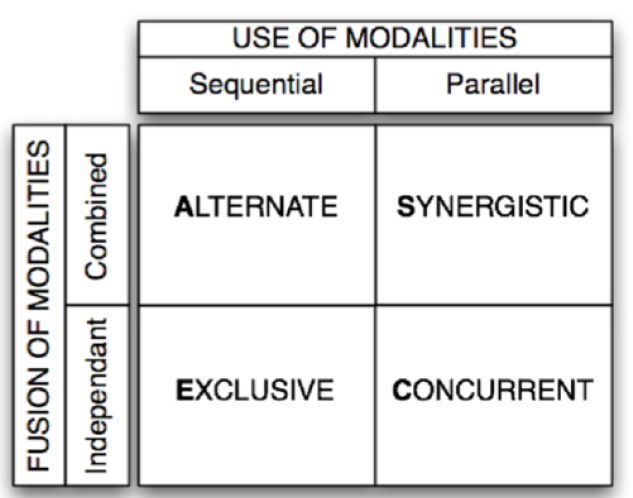
\includegraphics[scale=0.9]{casecare}
\caption{The CASE model}
\label{case-model}
\end{figure}
\newline
The \textit{CASE} model classified the machine-side of the fusion, now the \textit{CARE} model is about the human-side of fusion and classifies the usability properties: in our application, the two modalities are complementary. We need to use both of them to use correctly the application. 

\subsection{Fusion and fission}
We use \textit{decision-level fusion}: we merge lately the two modalities (the gaze position and the key pressing) because they are weakly coupled. On the fission side, it is a bit hard to have two different outputs for the user: we kept the feedback visual by highlighting the gazed-at element and by letting the menus appear directly upon a key press.  

\section{Architecture}

\subsection{Hardware}
The only specific hardware we use is the \textit{Tobii Eye Tracker 4C}. It is a small device that can be fixed on your monitor and plugged in a \textit{USB} port, on the form of a bar. It will then record the position of your eyes and the region of your screen you are gazing at. 

\subsection{Software}
To be able to access the \textit{Tobii} gaze data, we used the \textit{Tobii Core Standard Development Kit}\footnote{https://developer.tobii.com/tobii-core-sdk/} and its provided \textit{API}s. We then decided not to implement a plugin for an already existing text editor but rather to create our own one. The \textit{Windows Presentation Foundation}\footnote{https://msdn.microsoft.com/fr-fr/library/aa970268(v=vs.100).aspx} was all we needed: windows creation with built-in text fields and style modification. The \textit{WPF} uses the \textit{XAML} language. 

\subsection{Implementation}


\section{Data analysis}

\subsection{Hypothesis}
We hope to see a significant amelioration in the text editing quality by using our application. Therefore we can formulate our null hypothesis as follows: 
\[H_0: \text{There is no increase in speed by editing text with the eye tracker.}\] 
along with the alternative hypothesis: 
\[H_1: \text{Editing text with eye tracker support is faster than without it.}\]

\subsection{Experiment}

\subsection{Analysis and results}

\section{Conclusion}
 
\end{document}

